\chapter{Apreciaciones generales.}
%
Las conclusiones se basan en el an\'alisis tomado de la matriz de asociaci\'on de poder e inter\'es 
(\ref{matrizstakeholders}), resultado de la encuesta realizada a los stakeholders involucrados (GESPRO04 - Registro 
de Stakeholders.pdf) en el proyecto (GESPRO05 - Encuesta y Matriz.pdf).\\
%
\begin{figure}[H]
    \centering
    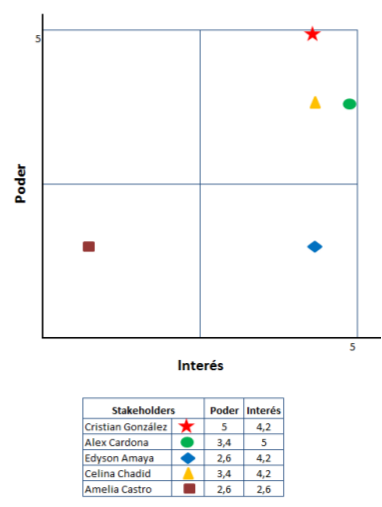
\includegraphics[width=0.95\textwidth]{images/matrizstakeholders.png}
    \caption{Matriz de clasificaci\'on de Stakeholders.}
    \label{matrizstakeholders}
\end{figure}
%
\chapter{STAKEHOLDERS}
%
\section{Cristian Gonz\'alez}
%
\noindent \textbf{Cargo:} Gerente General.\\
%
\textbf{Calificaci\'on poder:} 5.0\\
%
\textbf{Calificaci\'on inter\'es:} 4.2\\
%
\textbf{Impacto:} Alto.\\
%
\textbf{Conclusiones:}\\
%
\\Debido al rol que desempe\~na, es la persona con m\'as poder sobre la organizaci\'on; es el encargado
de la autorizaci\'on de adquisiciones y compras. Por otra parte, a diferencia de otros casos, tiene mucho 
inter\'es en la implementaci\'on de este proyecto, dado que le afecta directamente para la toma de decisiones
y la elaboraci\'on de planes estrat\'egicos dentro de la organizaci\'on.\\
%
\section{Alex Cardona}
%
\noindent \textbf{Cargo:} Gerente Administrativo y financiero.\\
%
\textbf{Calificaci\'on poder:} 3.4\\
%
\textbf{Calificaci\'on inter\'es:} 5.0\\
%
\textbf{Impacto:} Alto.\\
%
\textbf{Conclusiones:}\\
%
\\Aunque no posea voto en la toma de decisiones, su impacto afecta el proyecto debido a que su rol es indispensable
en el acompa\~namiento para la elaboraci\'on de los planes estrat\'egicos y por eso, es que demuestra gran
inter\'es en la implementaci\'on del mismo. Se recomienda tener en cuenta de forma particular todas sus 
inquietudes.\\
%
\section{Edyson Amaya}
%
\noindent \textbf{Cargo:} Gerente de producci\'on.\\
%
\textbf{Calificaci\'on poder:} 2.6\\
%
\textbf{Calificaci\'on inter\'es:} 4.2\\
%
\textbf{Impacto:} Medio.\\
%
\textbf{Conclusiones:}\\
%
\\Aunque no posea voto en la toma de decisiones, su impacto afecta el proyecto debido a que su rol es indispensable
en el acompa\~namiento para la elaboraci\'on de los planes estrat\'egicos y por eso, es que demuestra gran
inter\'es en la implementaci\'on del mismo. Se recomienda tener en cuenta de forma particular todas sus 
inquietudes.\\
%
\section{Celina Chadid}
%
\noindent \textbf{Cargo:} Gerente de recursos humanos.\\
%
\textbf{Calificaci\'on poder:} 3.4\\
%
\textbf{Calificaci\'on inter\'es:} 4.2\\
%
\textbf{Impacto:} Alto.\\
%
\textbf{Conclusiones:}\\
%
\\Aunque no posea voto en la toma de decisiones, su impacto afecta el proyecto debido a que su rol es indispensable
en el acompa\~namiento para la elaboraci\'on de los planes estrat\'egicos y por eso, es que demuestra gran
inter\'es en la implementaci\'on del mismo. Se recomienda tener en cuenta de forma particular todas sus 
inquietudes.\\
%
\section{Amelia Castro}
%
\noindent \textbf{Cargo:} Gerente comercial.\\
%
\textbf{Calificaci\'on poder:} 2.6\\
%
\textbf{Calificaci\'on inter\'es:} 2.6\\
%
\textbf{Impacto:} Bajo.\\
%
\textbf{Conclusiones:}\\
%
\\Su rol no implica voz ni voto en la toma de decisiones a nivel gerencial; su compromiso con los planes
estrat\'egicos est\'a al mismo nivel que el de todos en la empresa: comprometidos en la colaboraci\'on general.
Su nivel de inter\'es sobre el proyecto es bajo porque no requiere muchas de las funcionalidades ofrecidas.\\